% Main figures with formal submission captions.
% Source PNGs live in ../outputs/figures/.

\section*{Main Figures}

\begin{figure}[p]
  \centering
  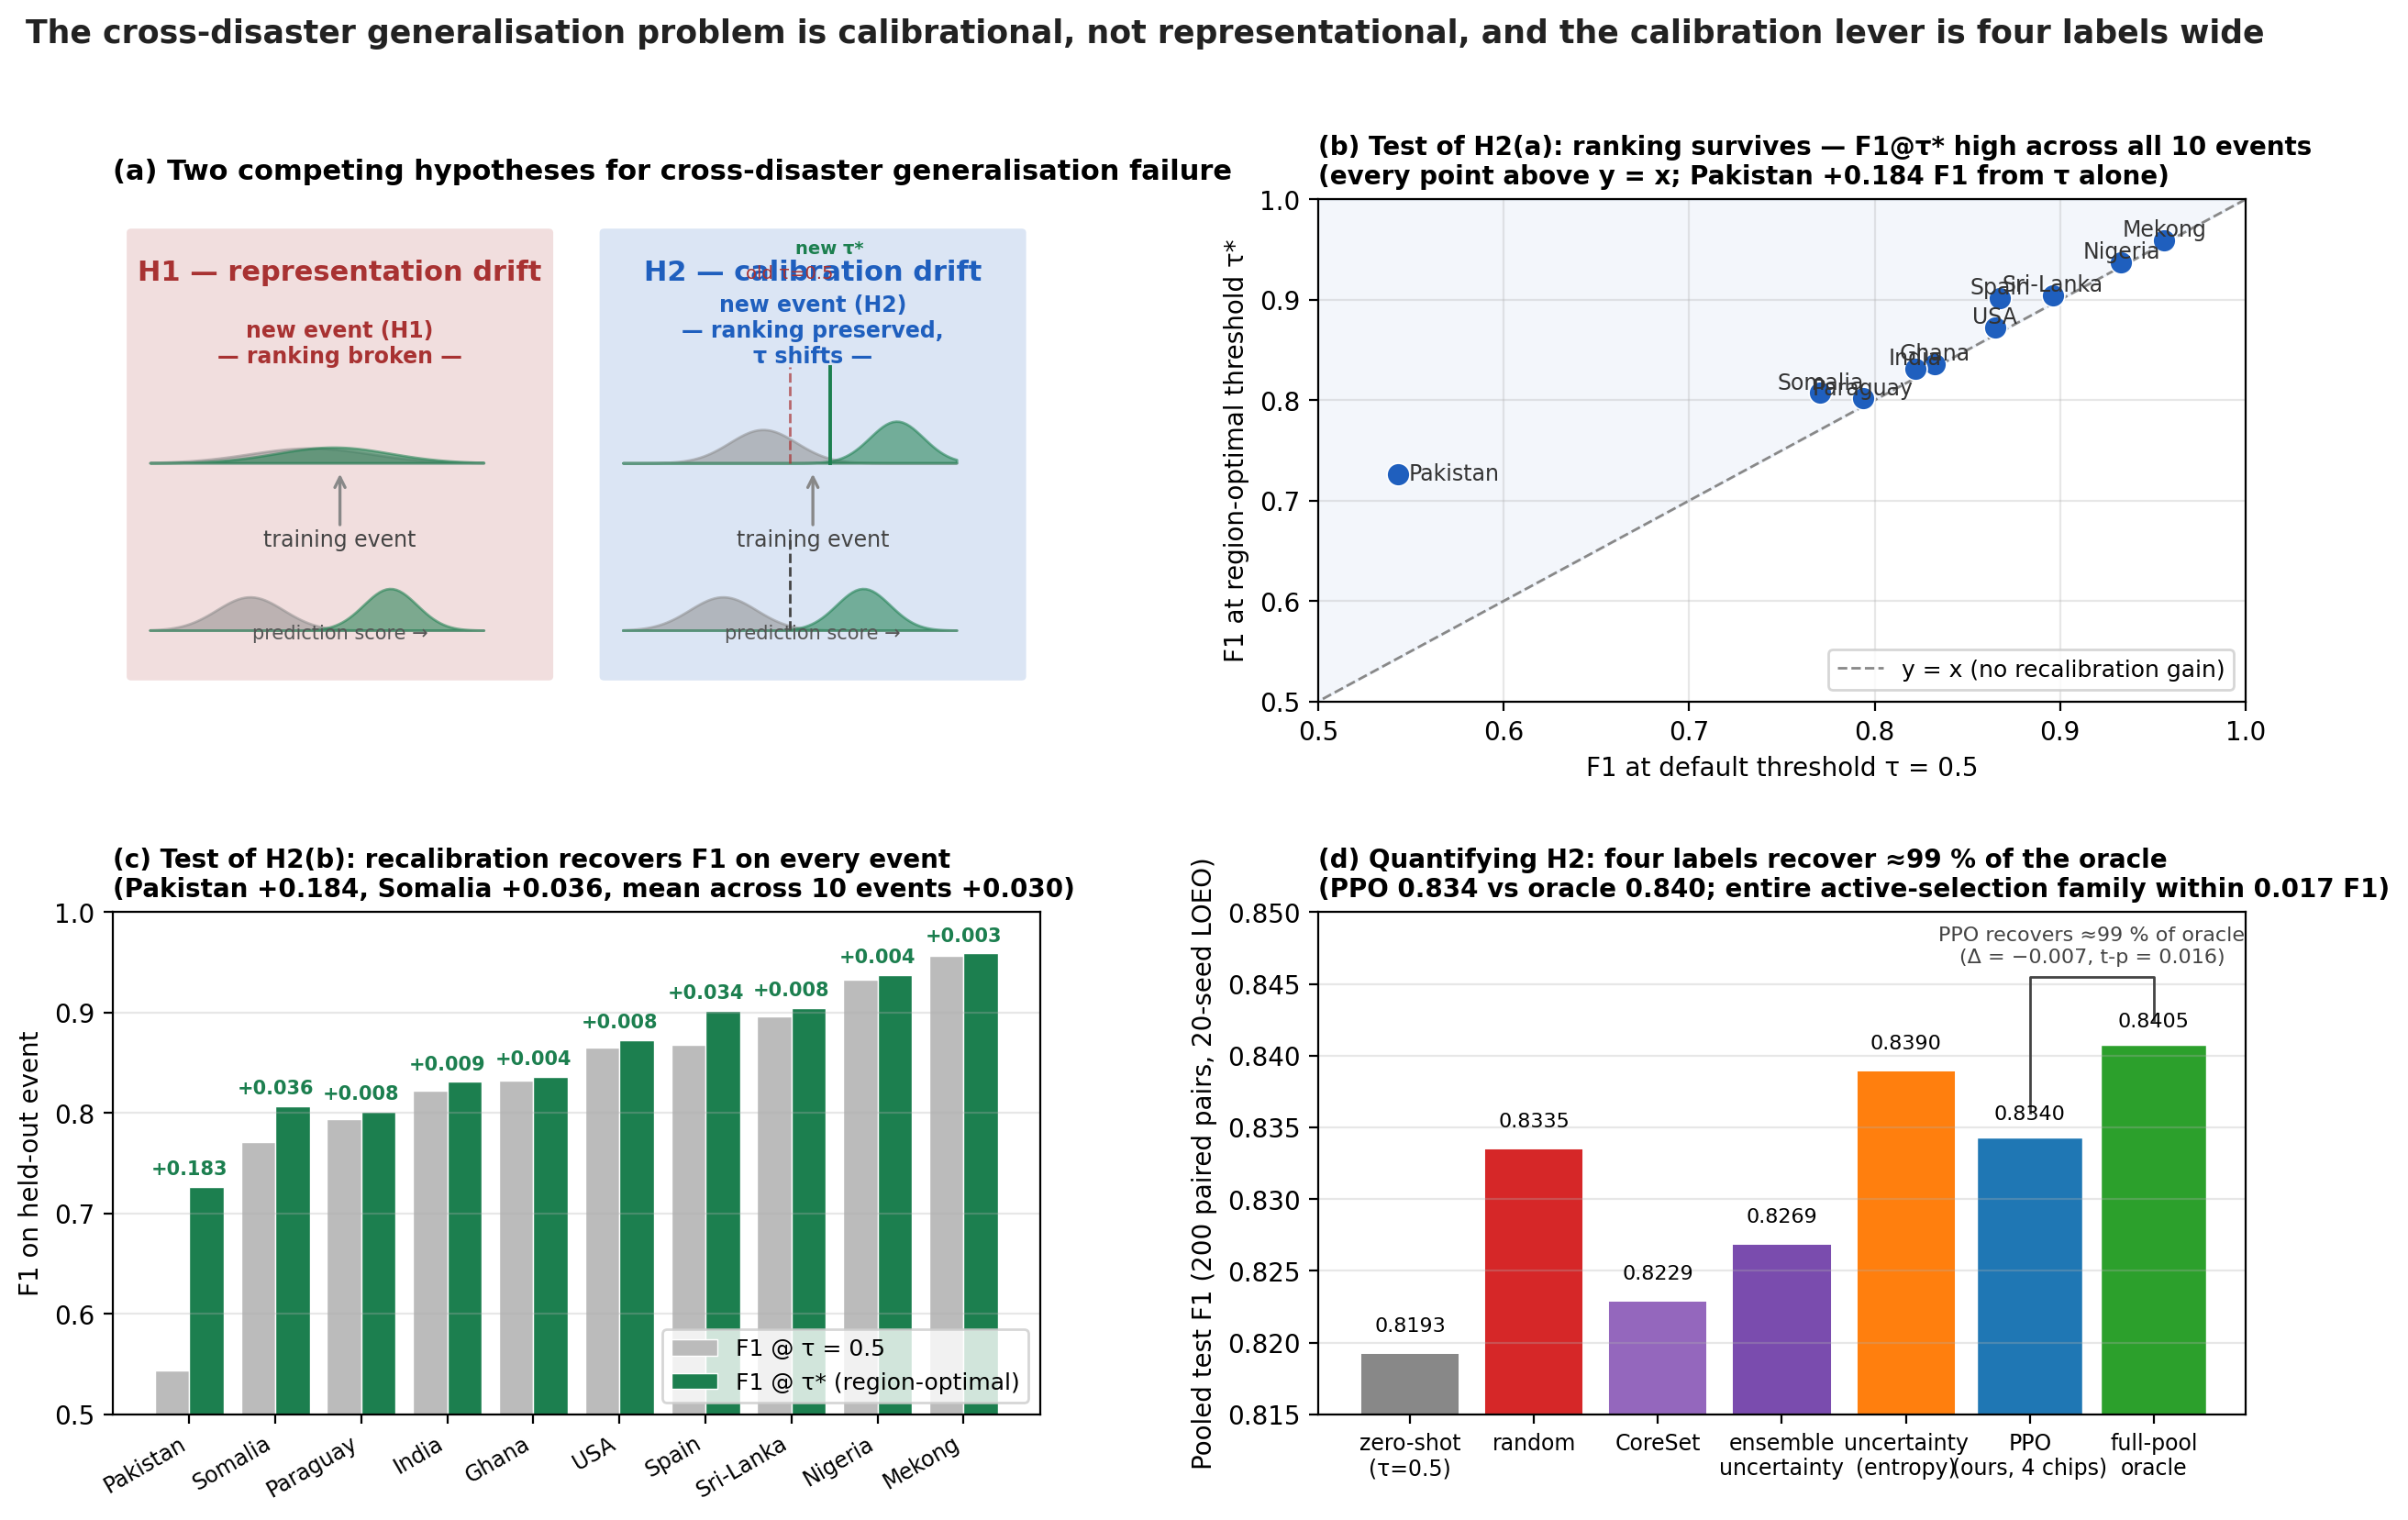
\includegraphics[width=\textwidth]{../outputs/figures/fig1_h1_h2_concept.png}
  \caption{\textbf{Two competing hypotheses for cross-disaster
  generalisation failure, and the experiments that discriminate them.}
  \textbf{a}, Conceptual schematic. Under representation drift (H1, red)
  the per-class score distributions of a model applied to a new event
  collapse onto one another --- the pixel ranking itself breaks, and no
  threshold can recover performance. Under calibration drift (H2, blue)
  the per-class distributions retain their shape but translate along the
  score axis --- the ranking is preserved and a single threshold
  adjustment (from the training value $\tau=0.5$ to the event-optimal
  $\tau^{*}$) recovers performance. \textbf{b}, Test of H2(a): F1 at the
  event-optimal threshold versus F1 at the default threshold for the ten
  Sen1Floods11 flood events; every point lies above the identity line
  (Pakistan +0.184 F1 from the threshold alone). \textbf{c}, Test of
  H2(b): per-event F1 at $\tau=0.5$ (grey) versus $\tau^{*}$ (green),
  annotated with the recoverable calibration gain. \textbf{d},
  Quantifying H2: pooled test F1 across 200 leave-one-event-out paired
  pairs for seven calibration strategies; a four-chip calibration set
  recovers $\approx99\,\%$ of the full-pool oracle's F1 regardless of
  the selection method.}
  \label{fig:concept}
\end{figure}

\begin{figure}[p]
  \centering
  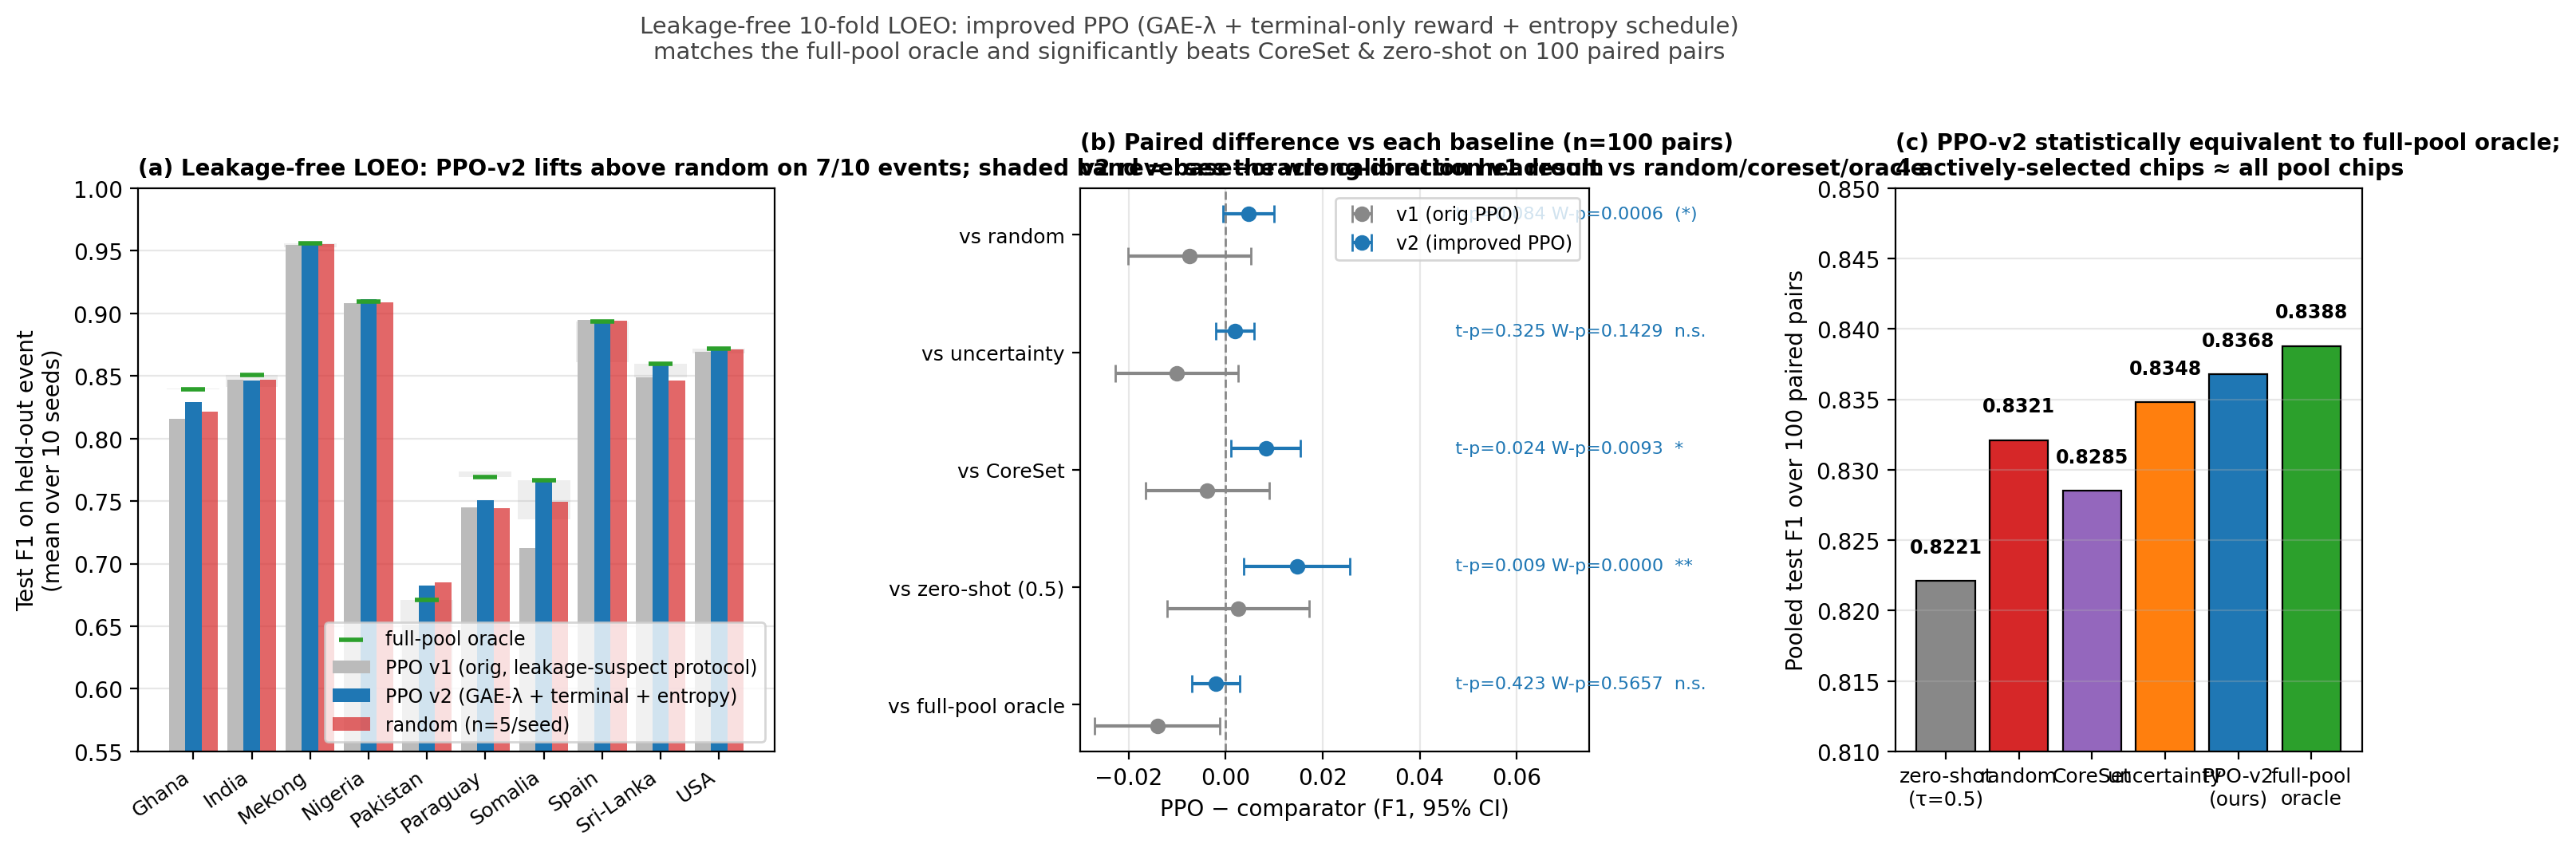
\includegraphics[width=\textwidth]{../outputs/figures/fig26_loeo_v1_v2.png}
  \caption{\textbf{Leakage-free leave-one-event-out evaluation of active
  threshold calibration.} \textbf{a}, Per-event test F1 of the learned
  PPO policy before (v1, grey) and after (v2, blue) the three structural
  corrections (GAE-$\lambda$ credit assignment, episode-terminal reward,
  entropy schedule), against four-chip random calibration (red) and the
  full-pool oracle (green dashes); shaded bands show the base-to-oracle
  calibration headroom per event. \textbf{b}, Pooled paired differences
  (PPO minus comparator) with 95\,\% confidence intervals across the
  leave-one-event-out protocol. \textbf{c}, Pooled F1 ladder across all
  methods. The five practical 4-chip selection methods span only
  0.017~F1 --- an order of magnitude smaller than the single-event
  calibration drift (up to +0.235~F1) that any of them corrects.}
  \label{fig:loeo}
\end{figure}

\begin{figure}[p]
  \centering
  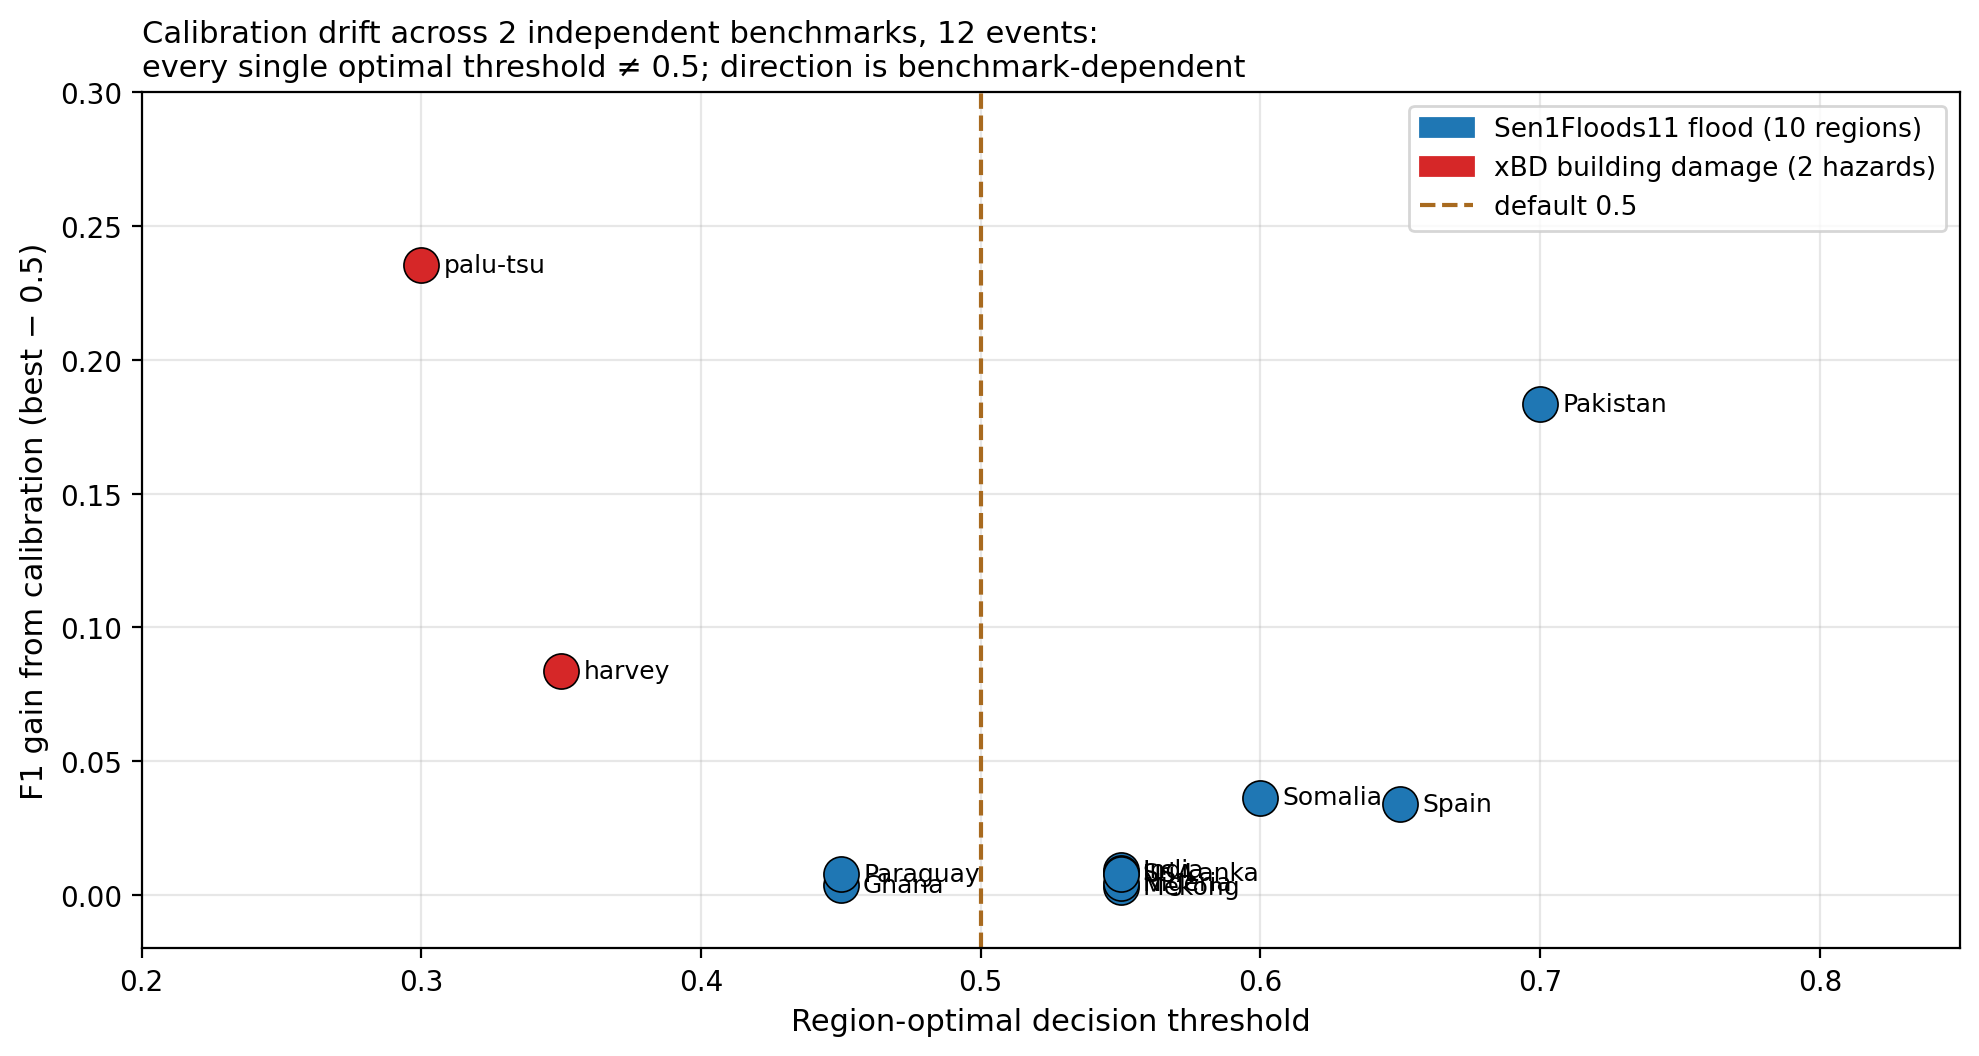
\includegraphics[width=\textwidth]{../outputs/figures/fig22_calibration_cross_benchmark.png}
  \caption{\textbf{Calibration drift across benchmarks and hazard
  families.} Event-optimal decision thresholds $\tau^{*}$ and the F1
  recovered by threshold re-fitting alone, for Sen1Floods11 floods and
  xBD building damage (HLS Burn-Scars wildfires reported in
  Results~R3). The direction of drift is benchmark-specific (floods
  drift up, damage drifts down) and the magnitude is hazard-specific
  (large for floods and damage, small for wildfires), but 15 of the 16 events with
  measured event-optimal thresholds differ from the 0.5 default.}
  \label{fig:crossbench}
\end{figure}

\begin{figure}[p]
  \centering
  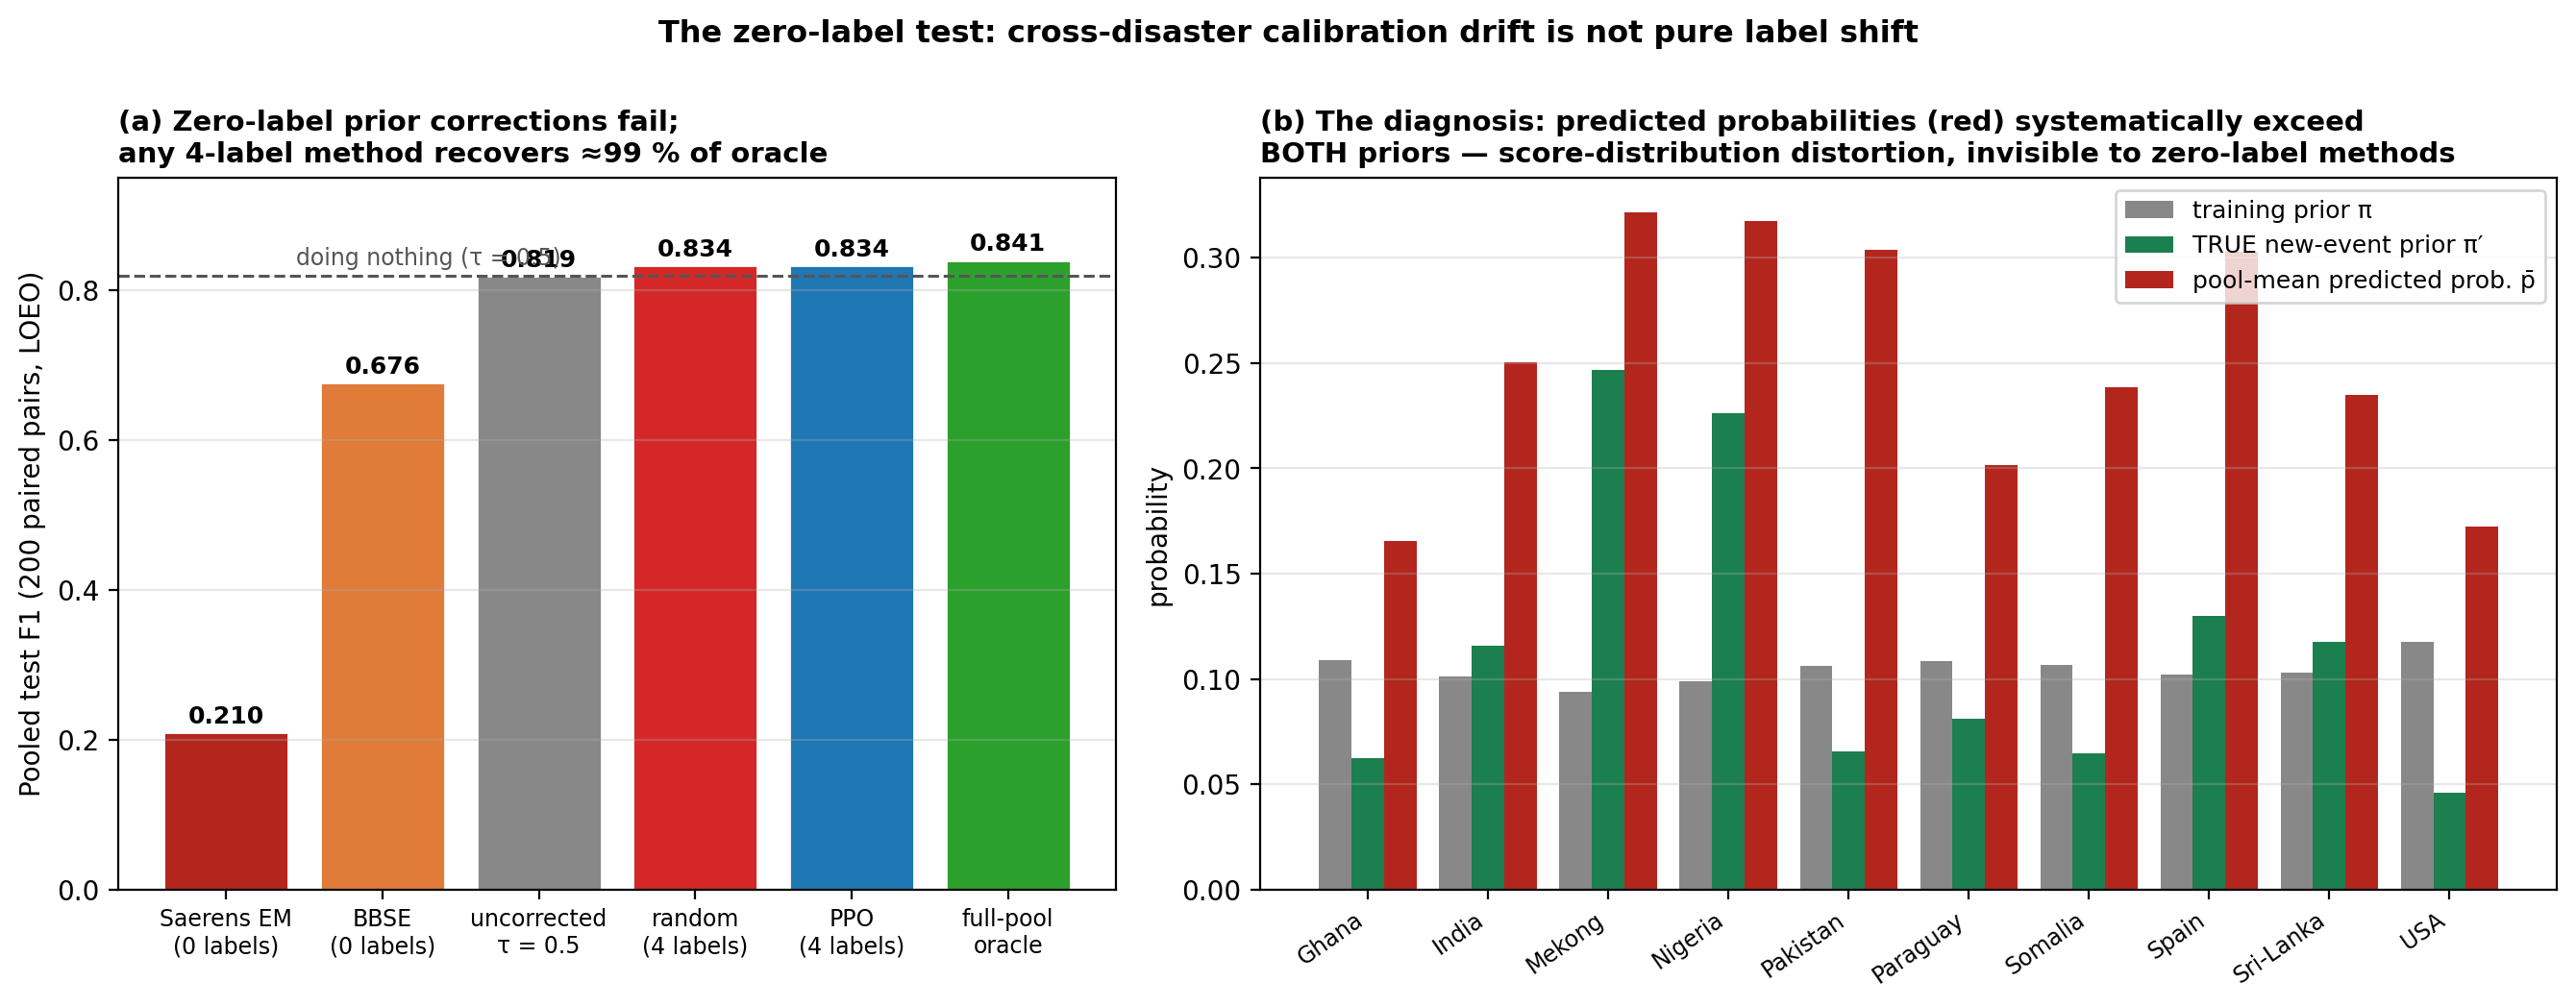
\includegraphics[width=\textwidth]{../outputs/figures/fig29_zero_label_test.png}
  \caption{\textbf{The zero-label test: cross-disaster calibration drift
  is not pure label shift.} \textbf{a}, Pooled test F1 (200
  leave-one-event-out paired pairs) for the two standard zero-label
  prior-shift corrections --- Saerens expectation--maximisation (EM) and
  black-box shift estimation (BBSE) --- against the uncorrected default,
  four-label calibration, and the full-pool oracle. Both zero-label
  corrections fall \emph{below} doing nothing. \textbf{b}, The
  diagnosis: per event, the model's pool-mean predicted probability
  (red) systematically exceeds both the training prior (grey) and the
  \emph{true} new-event prior (green). The class-conditional score
  distributions distort under cross-event transfer; labels measure this
  distortion, which no zero-label method can see. BBSE estimates the
  new-event priors nearly correctly yet its analytically corrected
  threshold still fails, isolating score distortion --- not prior
  mis-estimation --- as the dominant failure mode.}
  \label{fig:zerolabel}
\end{figure}

\begin{figure}[p]
  \centering
  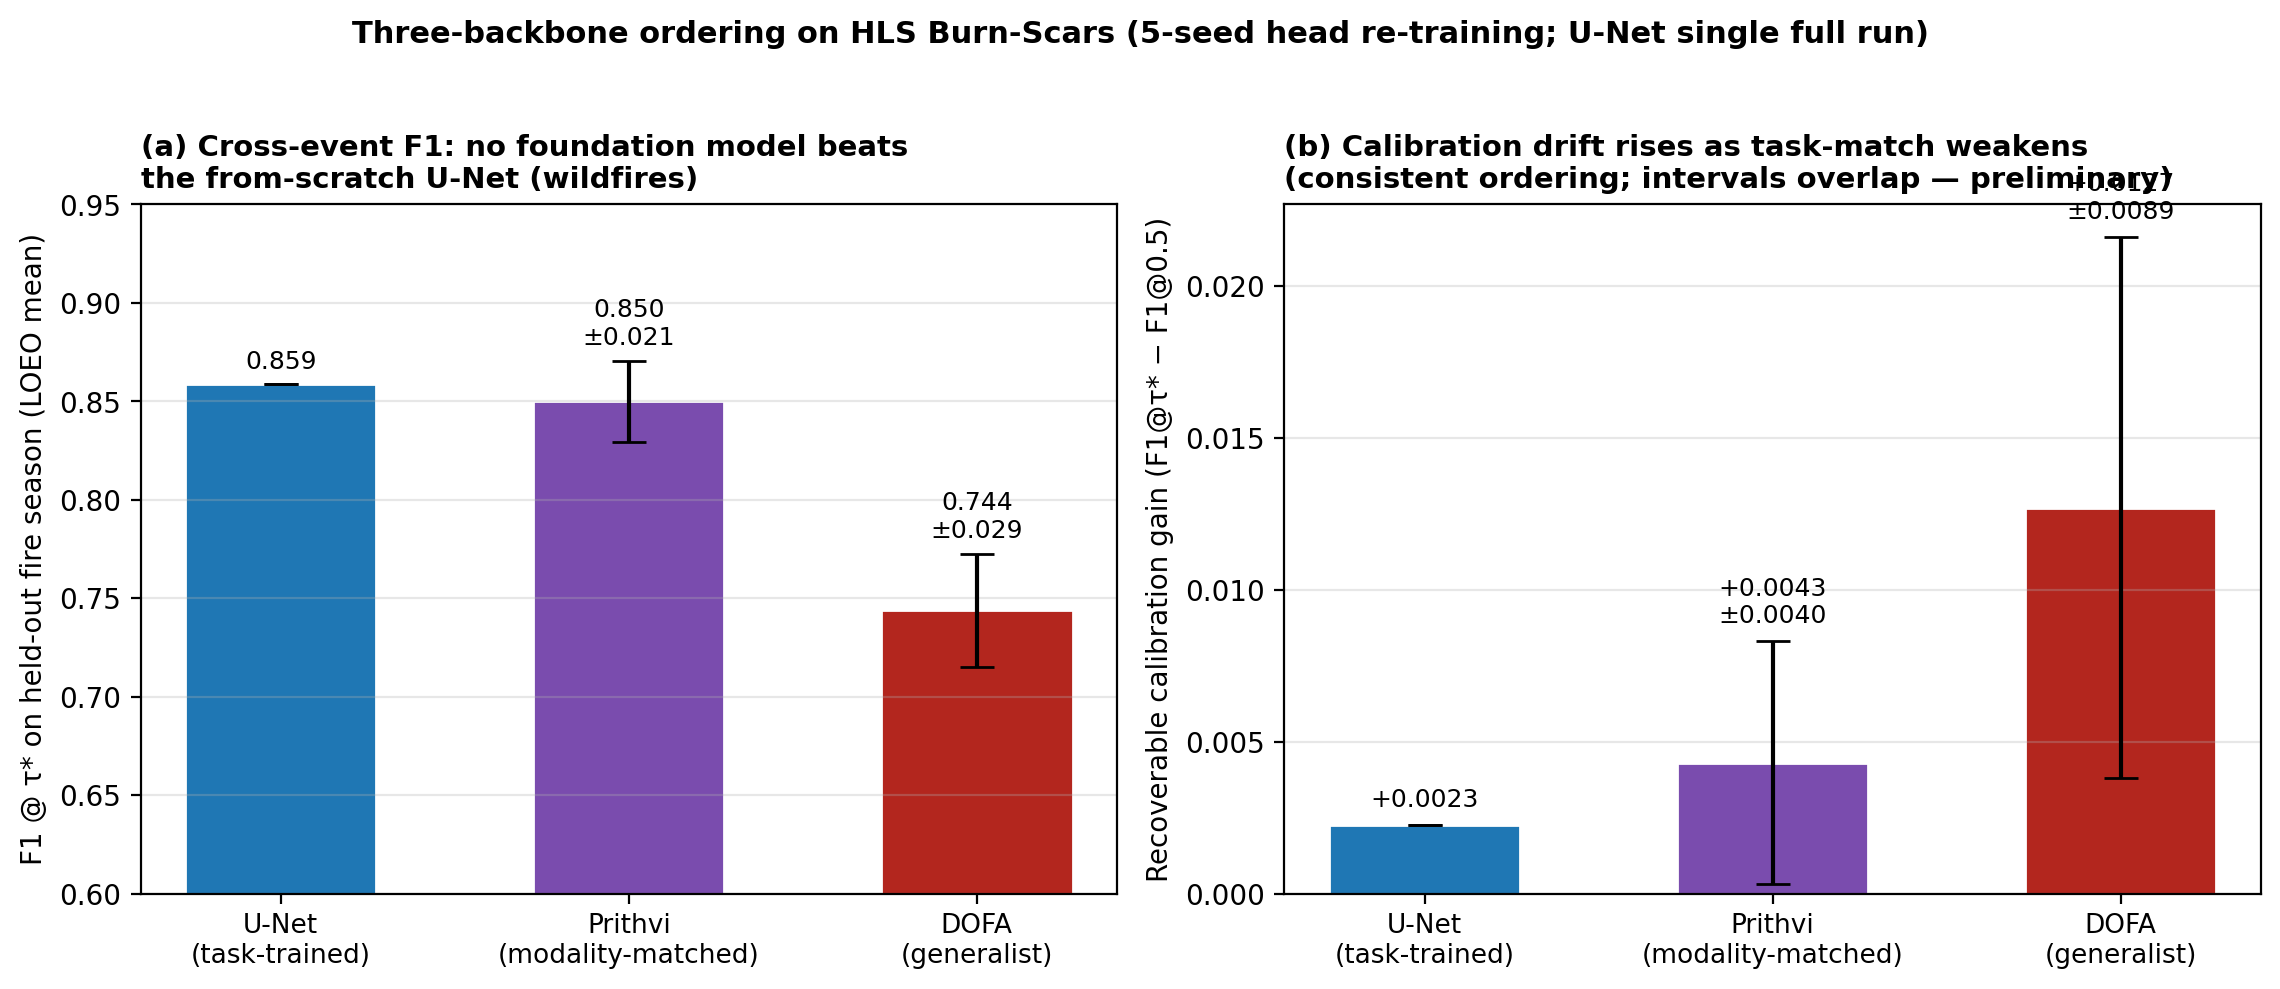
\includegraphics[width=0.92\textwidth]{../outputs/figures/fig30_backbone_ordering.png}
  \caption{\textbf{Three-backbone ordering on HLS Burn-Scars: weaker
  task-match, more calibration drift.} \textbf{a}, Cross-event F1 at the
  event-optimal threshold for a task-trained U-Net, the
  modality-matched Prithvi-EO-1.0-100M foundation model, and the
  generalist DOFA foundation model, under identical
  leave-one-fire-season-out protocols (foundation-model bars: mean
  $\pm$ s.d.\ over five segmentation-head training seeds on frozen
  encoder features; U-Net: single full training run per fold).
  \textbf{b}, Recoverable calibration gain per backbone. The ordering
  is consistent across seeds but adjacent intervals overlap; we present
  it as a consistent preliminary ordering rather than a statistically
  separated gradient.}
  \label{fig:backbones}
\end{figure}

\begin{figure}[p]
  \centering
  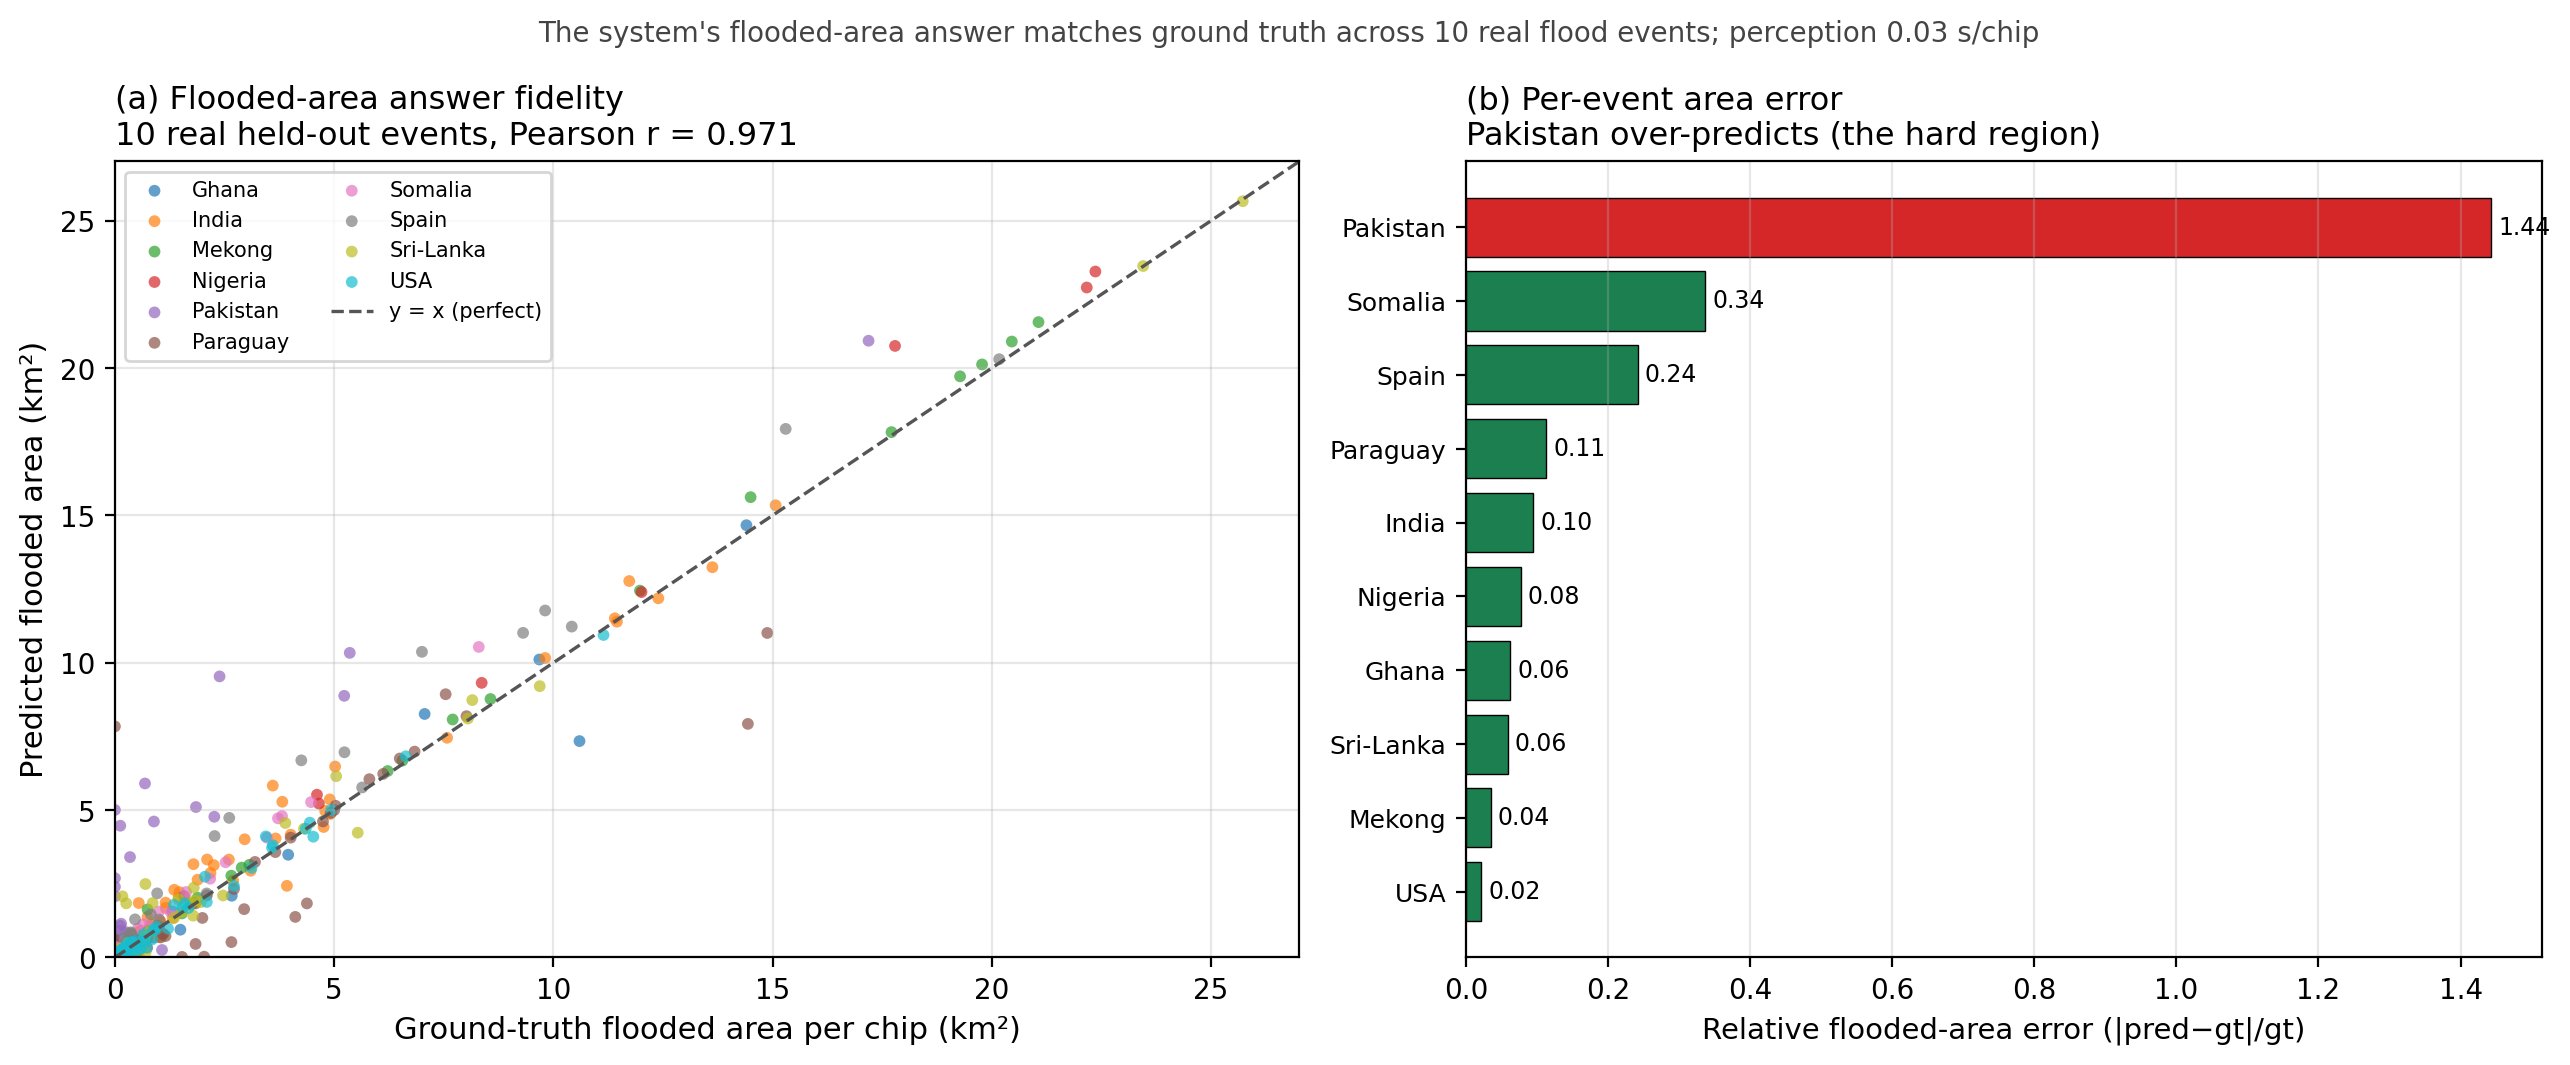
\includegraphics[width=\textwidth]{../outputs/figures/fig17_answer_fidelity.png}
  \caption{\textbf{End-to-end decision-level answer fidelity.}
  Flooded-area answers produced by the full perception $\rightarrow$
  calibration $\rightarrow$ reasoning agent against analyst hand-labels
  across 431 chips spanning ten real flood events (Pearson
  $r=0.971$; Spearman $\rho=0.899$; median absolute percentage error
  25\,\%). The Pearson headline is driven by the largest events
  (bottom-50\,\%-by-area chip $r=0.118$): the agent's totals are
  reliable in the event-ranking regime responders use, while
  small-area chips carry wide relative errors (Results~R1).}
  \label{fig:fidelity}
\end{figure}
